
%%%%%%%%%%%%%%%%%%%%%%% file typeinst.tex %%%%%%%%%%%%%%%%%%%%%%%%%
%
% This is the LaTeX source for the instructions to authors using
% the LaTeX document class 'llncs.cls' for contributions to
% the Lecture Notes in Computer Sciences series.
% http://www.springer.com/lncs       Springer Heidelberg 2006/05/04
%
% It may be used as a template for your own input - copy it
% to a new file with a new name and use it as the basis
% for your article.
%
% NB: the document class 'llncs' has its own and detailed documentation, see
% ftp://ftp.springer.de/data/pubftp/pub/tex/latex/llncs/latex2e/llncsdoc.pdf
%
%%%%%%%%%%%%%%%%%%%%%%%%%%%%%%%%%%%%%%%%%%%%%%%%%%%%%%%%%%%%%%%%%%%


\documentclass[runningheads,a4paper]{llncs}

\usepackage{amssymb}
\setcounter{tocdepth}{3}
\usepackage{graphicx}
\usepackage{times}
\usepackage{url}
\urldef{\mailsa}\path|{alfred.hofmann, ursula.barth, ingrid.haas, frank.holzwarth,|
\urldef{\mailsb}\path|anna.kramer, leonie.kunz, christine.reiss, nicole.sator,|
\urldef{\mailsc}\path|erika.siebert-cole, peter.strasser, lncs}@springer.com|
\newcommand{\keywords}[1]{\par\addvspace\baselineskip
\noindent\keywordname\enspace\ignorespaces#1}

\begin{document}

\mainmatter  % start of an individual contribution

% first the title is needed
\title{MixGF: spectral probabilities for mixture spectra from more than one peptide}

% a short form should be given in case it is too long for the running head
\titlerunning{Spectral probabilities for mixture tandem mass spectra}

% the name(s) of the author(s) follow(s) next
%
% NB: Chinese authors should write their first names(s) in front of
% their surnames. This ensures that the names appear correctly in
% the running heads and the author index.
%
\author{Jian Wang$^{1}$
\and Philip E. Bourne$^{2}$ \and Nuno Bandeira$^{2,3,4}$}
\authorrunning{MixGF: Spectral Probabilities for Mixture Tandem Mass Spectra}
% (feature abused for this document to repeat the title also on left hand pages)

% the affiliations are given next; don't give your e-mail address
% unless you accept that it will be published
\institute{$^{1}$Bioinformatics Program, University of California, San Diego, La Jolla, USA\\
$^{2}$Skaggs School of Pharmacy and Pharmaceutical Sciences, UCSD, San Diego, La Jolla, USA\\
$^{3}$Center for Computational Mass Spectrometry, University of California, San Diego, La Jolla USA \\
$^{4}$Department of Computer Science and Engineering, University of California, San Diego, La Jolla, USA\\
}

%
% NB: a more complex sample for affiliations and the mapping to the
% corresponding authors can be found in the file "llncs.dem"
% (search for the string "\mainmatter" where a contribution starts).
% "llncs.dem" accompanies the document class "llncs.cls".
%

%\toctitle{Lecture Notes in Computer Science}
%\tocauthor{Authors' Instructions}
\maketitle


\begin{abstract}
It is becoming increasingly recognized that in many large-scale proteomic experiments, multiple peptide precursors are often co-fragmented simultaneously in the same \emph{mixture} tandem mass (MS/MS) spectrum. These spectra tend to elude current computational tools because of their ubiquitious assumption that each spectrum is generated from only one peptide. Therefore tools that consider multiple peptide matches to each MS/MS spectrum can potentially improve the relatively low spectrum identification rate often observed in proteomics experiments. More importantly, data independent acquisition protocols are emerging as alternative methods that can greatly improve the throughput of peptide identifications but their success also depends on the availability of algorithms able to identify multiple peptides from each MS/MS spectrum.  Here we address a fundamental question in the identification of mixture MS/MS spectra: determining the statistical significance of multiple peptides matched to an MS/MS spectrum. We propose a generating function model to rigorously compute the statistical significance of peptide identifications for mixture spectra and show that this approach improves the sensitivity of state-of-the-art mixture spectra database search tools by 25\% - 160\%.

\keywords{Tandem mass spectrometry, mixture spectrum, statistical significance, database search, co-eluting peptides, data independent acquisition, generating function, proteomics}
\end{abstract}

\clearpage
\section*{Introduction}

In recent years, the advancement of technology and instrumentation has made tandem mass (MS/MS) spectrometry the leading high-throughput method to analyze proteins~\cite{washburn2001large,brunner2007high,aebersold2003mass}.  In typical experiments, tens of thousands to millions of MS/MS spectra are generated and enable researchers to probe various aspects of the proteome on a large scale.  Part of this success is hinged on the development of computational methods that can analyze the large amount of data generated from these experiments. The classical question in computational proteomics asks: given an MS/MS spectrum, what is the \emph{peptide} that generated the spectrum? However, it is increasingly being recognized that this assumption that each MS/MS spectrum comes from \emph{only one} peptide is often not valid.  As instruments with high mass accuracy enable better distinction between peptides with close precursor masses, several recent analyses show that as many as 50\% of the MS/MS spectra collected in typical proteomics experiments come from more than one peptide precursor~\cite{pr101060v,pr800307m}. The presence of multiple peptides in mixture spectra can decrease their identification rate to as low as one half of those MS/MS spectra generated from only one peptide~\cite{gelio2008detect,houel2010quant,wang2011peptide}. In addition, there have been numerous developments in Data Independent Acquisition (DIA) technologies where multiple peptide precursors are purposefully selected to co-fragment in each MS/MS spectrum~\cite{masselon2003itp,venable2004aaq,plumb2006uplc,chakraborty2007uim,panchaud2009precursor,michalski2011mass,2012targeted}.  These emerging technologies can address some of the enduring disadvantages of traditional data-dependent acquisition methods (e.g. reproducibility of data) and can potentially increase the throughput of peptide identification 10--20 fold~\cite{pr101060v,blackburn2010improve}. However despite the growing importance of mixture spectra in various contexts, there are only a few computational tools that can analyze mixture spectra from more than one peptide~\cite{zhang2005tree,li2009database,bern2009deconvolution,wang2010msplit,wang2011peptide}.

In their pioneering work Zhang et. al. described the first database search method for mixture spectra, ProbIDtree~\cite{zhang2005tree} and showed that it is possible to identify co-eluting peptides from single MS/MS spectra. However ProbIDtree's accuracy for identifying mixture spectra is relative low compared to the accuracy of current database search methods in identifying single-peptide spectra~\cite{wang2011peptide}. Recently we proposed the first spectral library search method (M-SPLIT~\cite{wang2010msplit}) and a new database search method (MixDB~\cite{wang2011peptide}) for identification of mixture spectra and show that these can be identified efficiently with accuracy comparable to that of single-peptide spectra.  Further analysis of the results between  spectral library and database search methods reveals that current database search methods still suffer from relative low sensitivity due to their limited ability to separate true matches from false positive matches - still an open research problem even for the case of single-peptide spectra~\cite{kall2007semi,kim2008spectral,nesvizhskii2010survey}.  Capitalizing on recent advances on using a generating function approach to rigorously compute the statistical significance of peptide-spectrum matches (PSMs), we extended this MS-GF~\cite{kim2008spectral} approach and show how to rigorously compute statistical significance for peptide identification with mixture spectra.  Applying this approach (MixGF) on both simulated and real datasets, we show that MixGF improves the sensitivity of identification of mixture spectra by 26-76\% over MixDB~\cite{wang2011peptide} and by 110-162\% over ProbIDtree~\cite{zhang2005tree}.

\clearpage

\section*{Method}
\subsection*{Scoring function for mixture spectrum}
We represent a tandem mass (MS/MS) spectrum with parent mass N, as a real-valued vector: $V = v_{1} ... v_{N}$ with N elements, where $v_{i}$ is the sum of intensity of all the peaks with mass between i-0.5 and i+0.5. A prefix residue mass (PRM) spectrum is a transformation of an observed MS/MS spectrum into a scored version $S = s_{1} ... s_{N}$ using a probabilistic model as described before~\cite{kim2009}.  At every mass position $i$ of the PRM spectrum is a score $s_{i}$ that represents the log-likelihood that the peptide from which the spectrum was generated contains a prefix mass $i$~\cite{dancik99}. Given a peptide P, its prefix masses are defined by the sum of amino acid masses for each peptide prefix.  For a peptide P with prefix masses $p_{1} .... p_{n}$, we define its parent mass as $p_{n}$ and the score of matching peptide P to a spectrum is the sum of all the scores at its theoretical prefix masses in the PRM spectrum: SCORE(P) = $s_{p_{1}} + s_{p_{2}} ... + s_{p_{n}}$.

We define a mixture spectrum as an MS/MS spectrum from two different peptides. When interpreting an MS/MS spectrum as a mixture spectrum $M$, we construct two PRM spectra, $M^{H}$ and $M^{L}$, to represent the two scoring models for the high and low-abundance peptides present in the mixture spectrum, respectively.  As we showed before~\cite{wang2011peptide}, different scoring models are needed for high and low-abundance peptides because they have quite distinct fragmentation statistics in mixture spectra.  Without loss of generality, when matching a mixture spectrum (M) against a pair of peptides (P, Q) we always assume the first peptide is the high-abundance peptide.  Thus the score of a pair of peptides (P, Q) against a mixture spectrum M will be the sum of scoring P with $M^{H}$ and scoring Q with $M^{L}$: SCORE(M, P, Q) = $M^{H}_{p_{1}} + ... M^{H}_{p_{n}} + M^{L}_{q_{1}} + ... M^{L}_{q_{n}}$. To avoid double counting, when a prefix mass of P is the same as a prefix mass of Q, only the bin with the higher score is considered and the other peptide gets a score of zero for that particular mass position:
$when\ p_{i} == q_{j}:$
$ if(M^{H}_{p_{i}} > M^{L}_{q_{j}})
  \{ M^{L}_{q_{j}} = 0 \}
 else \{ M^H_{p_{i}} = 0 \}$.

\subsection*{Spectral probability for a mixture spectrum}
As described in Kim et. al., 2008~\cite{kim2008spectral}, the statistical significance of a particular peptide P matched to a spectrum S with score T is determined by the probability that a random peptide (out of all possible peptides) when matched to S has a score greater or equal to T. From hereon we will refer to this as the \emph{Single-peptide probability} in order to better distinguish it from the other definitions introduced below.   Analogously, to compute the statistical significance of a particular peptide pair (P,Q) matched to a mixture spectrum (M) with a score of T, we are interested in two statistical questions: 1)\emph{Joint-probability}: What is the probability that a random peptide pair (out of all possible peptide pairs) when matched to M yields a score greater or equal to T? and 2) \emph{Conditional-probability}: Given a peptide P, what is the probability that a random peptide Q (out of all possible peptides) together with P when matched to M yields a score greater or equal to T?  Intuitively we are interested in finding cases where both peptides P and Q are statistically significant matches to a spectrum M. We address this question in two steps.  \emph{Joint-probability} assesses the chance that two random peptides can have the same or higher score than the current best match.  When this probability is very low, this means that at least one peptide is a significant match to the spectrum. Once we assume that at least one peptide is a true match, \emph{Conditional-probability} helps us evaluate whether the second peptide is also a statistically significant match.

In order to compute the score distribution for all peptides, MSGF~\cite{kim2008spectral} uses a dynamic programming approach to compute the Single-peptide probability efficiently without explicitly computing the scores for all peptides.  Here we extend this generating function approach to compute the probability for \emph{Joint} and \emph{Conditional} probabilities. \\
Let $J_M(p_{i}, q_{j}, T)$ be the Joint-probability that a pair of peptides $P$, $Q$ with parent mass $p_{i}$ and $q_{j}$ match to M with score higher than or equal to T. Also recall that $M^{H}$ and $M^{L}$ represent the PRM spectra for the high and low abundance peptides, respectively.  Then we can define the following recurrence relationship for Joint-probability: \\
\\
\\
$J_M(p_{i},q_{j},T) = \left\{
\begin{array}{l}
  if\ p_{i} < q_{j}: \\
      \displaystyle\sum\limits_{all\ amino\ acids\ a}{J_M(p_{i}, q_{j} - |a|, T - M^{L}(q_{j}))\times prob(a)} \\
  if\ p_{i} > q_{j}:\\
      \displaystyle\sum\limits_{all\ amino\ acids\ a}{ J_M(p_{i} - |a|, q_{j}, T - M^{H}(p_{i}))\times prob(a)} \\
  if\ p_{i} == q_{j}: \\
  \sum\limits_{a_1}{\sum\limits_{a_2}{J_M(p_{i} - |a_1|, q_{j} - |a_2|,
        T - max \left\{
                  \begin{array}{c}
                   M^{H}(p_{i}) \\
                   M^{L}(q_{j})
                  \end{array}
                 \right\})}} \\
                 \ \ \ \ \ \ \ \ \ \ \times prob(a_1) \times prob(a_2)
\end{array}
\right\}
$
\\
\\
\\
In the equation above $a$, $a_1$, and $a_2$ denotes all possible amino acid residues; $|a|$ denotes the mass of an amino acid residue and prob($a$) denote the probability that a particular amino acid residue occurs in a peptide.  When considering all possible peptide sequences this probability is uniform and has a value of $\frac{1}{20}$ for all standard 20 amino acids. To better reflect the amino acid composition observed in real protein sequences we can also obtain this probability by computing the frequency of each amino acid residue in the protein sequence database against which the MS/MS spectra are searched.  To start the computation of the recurrence, we initialize $J_M(0,0,0)=1$.

The computation of the Conditional-probability is very similar to that of Single-peptide probability, except that it is conditioned on the first peptide being accepted as a match thus when a prefix mass of the second peptide is equal to a prefix mass of the first peptide, one only uses the score of the mass position with higher score.  More concretely, for a peptide pair ($P$, $Q$) matched to spectrum $M$ with score $T$, let's assume peptide P and Q contribute $T_{P}$ and $T_{Q}$ to the total score respectively. Given that peptide P matches to M, we define $C_M(q_{j}, T | P)$ as the Conditional-probability that a peptide with parent mass $q_{j}$ together with P match to M results in higher than equal to T. To compute this probability, we first modify the PRM spectrum for the second peptide as follows:
$when: p_{i} == q_{j}\ \ \ \ M^{L}(q_{j}) = 0\ \ if\ M^{L}(q_{j}) < M^{H}(p_{i})$ \\
then the Conditional-probability is given by the following recurrence: \\
\vspace{2cm}
$C_M(q_{j},T | P) = \sum\limits_{all\ amino\ acids\ a}{C_M(q_{j} - |a|, T - M^{L}(q_{j}) | P)}\times prob(a)$ \\
We initialize the recurrence with the base case: $C_M(0, T_{P} | P) = 1$.  The base case starts at score $T_{P}$ rather than zero because the first peptide $P$ already contributes $T_{P}$ to the total score.

We note that even though the Joint-probability assesses whether at least one peptide is a significant match to the spectrum, it does not determine which peptide is the significant match.  More importantly, when calculating the Conditional-probability one assumes that the first peptide is a true match but it is unclear which peptide is the first peptide from the Joint-probability assessment. In order to resolve this ambiguity, for a candidate peptide pair ($P$,$Q$) matched to a spectrum $M$, we compute their respective Single-peptide probabilities and the peptide with lower (i.e. statistically more significant) Single-peptide probability is designated as the first peptide.

\subsection*{Approximating joint probability}
The dynamic programming approach above enables us to compute the \emph{Joint-probability} without explicitly computing the scores for all peptide pairs. However the computational complexity still scales exponentially with the number of peptides that possibly generated the observed spectrum (e.g., quadratic for two peptides).  Thus it is desirable to find a way to approximate this probability efficiently. To derive this approximation we borrow an intuition from the definition of conditional probability where the joint probability of two random events (P,Q), is equal to the probability of one event times the conditional probability of the second event given the first event: $Prob(P\ \wedge\ Q) = Prob(P)\times Prob(Q|P)$. Analogously we can decompose the Joint-probability question into two simpler questions: 1) what is the probability of finding a random peptide that matches to M with a score equal or better than $T_{P}$? and 2) once we find a first peptide $P$ what is the probability of finding a random peptide that together with $P$ scores equal or higher than $T$ when matched to M?  Note that the first question is just the \emph{Single-peptide probability} and the second question can be answered with the \emph{Conditional-probability}. Therefore we can define the following approximation:
$J_M(P,Q,T) \approx Single_M(P,T_{P}) \times C_M(Q,T| P)$. From hereon we refer to this approximation as the \emph{Product-probability}.
While this formulation is not exactly equivalent to the definition of Joint-probability (because it does not explicitly consider the dependencies between {\em all} possible pairs of peptides that can be matched to the mixture spectrum), both Single-probability and Conditional-probability can be computed efficiently in linear time and we show in the next section that this approximation is sufficiently accurate for our main use Joint-probability -- to separate correct matches from false positive matches.
%From a practical perspective, we are particularly interested the tail of this score distribution. In another word one wants to compute this probability accurately when the the score T is high.  We argue that when T is high, all the peptide pairs (A,B) with score higher than T should have individual score similar or better than those of P and Q: \\
%If $SCORE(A,B,M) > SCORE(P,Q,M)$ then with high probability: \\
%$SCORE(A,M)\geq T_{P}$ and $SCORE(B,M)\geq T_{Q}$.\\
%The intuition behind this is that when the combined score T is high, if one peptide has substantially lower score than P and Q, then the other peptide must score substantially higher to compensate for this and the probability of finding such a peptide which essentially has score as high as two correct peptide match is rare. This enable us to formulate the joint-probability question in a slightly different way: what is the probability of finding a peptide random A such that it score higher than $T_{P}$ and given that we have peptide A what is the probability of finding a second peptide B that together score higher than $T$.  Note that the first question is just the \emph{Single-peptide probability} and the second question can be approximated by the \emph{Conditional-probability}, both of which we know how to compute efficiently. Note that to answer the second question exactly we need to iterate over all possible peptides with score greater than $T_{P}$, while the Conditional-probability is conditioned on a particular peptide $P$, thus it is only an approximate answer to the second question.  Therefore we have:\\
%$J(P,Q,M,T) \approx Single(P,M,T_{P}) \times C(Q,M,T| P)$\\
%From hereon we refer to this approximation as the \emph{product-probability}.

\subsection*{Estimation of False Discovery Rates}
False Discovery Rate (FDR) can be estimated by extending the Target-Decoy Approach (TDA) for database search~\cite{elias07}. Each top scoring peptide-peptide-spectrum match (PPSM) can be one of the following type: \emph{TT} -- both peptide matches are from the target database, \emph{TD} or \emph{DT}  -- one peptide is from the target while the other peptide is from the decoy database and \emph{DD} -- both peptides are from the decoy database. A peptide from the target database can be either a correct (C) or incorrect match (I) and a peptide from a decoy database is by definition an incorrect match. Therefore we can write the number of PPSMs in each category as a sum of its subtypes:
\begin{eqnarray}
TT &=& CC^{TT} + CI^{TT} + IC^{TT} + II^{TT} \\
TD &=& CI^{TD} + II^{TD}  \\
DT &=& IC^{DT} + II^{DT}  \\
DD &=& II^{DD}       
\end{eqnarray}
TDA assumes that an incorrect match has equal chance of matching to target and decoy. Thus matches of II type has equal chance of being TT, TD, DT and DD, making the number of II matches in equation 1-4 the same: $DD = II^{DD}=II^{TD}=II^{TT}$.  By similar argument, the number of matches of type CI in equation 2 and the number of matches of type IC in equation 3 should be the same as those in equation 1. By substitution and rearranging terms, we can then redefine CI and IC in equation 1 to be: $CI^{TT} = TD - DD$ and $IC^{TT} = DT - DD$.  

The false discovery rate of PPSMs, which is the fraction false positive IDs in the TT category, can be defined as: $FDR_{matches} = \frac{1/2(IC^{TT}+CI^{TT}) + II^{TT}}{TT}$. The $1/2$ in the equation accounts for the fact that matches of IC and CI type contribute one correct match and one incorrect match. Substituting the terms defined above, we get:
\begin{eqnarray}
FDR_{matches} = \frac{1/2((TD-DD) + (DT -DD))+ DD}{TT} 
              = \frac{1/2(TD+DT)}{TT}   
\end{eqnarray}

\subsection*{Database search of mixture spectra}
Simulated mixture spectra were created as described before~\cite{wang2010msplit} by linearly combining two single-peptide spectra with mixture coefficients selected from 0.1 to 1.0. Mixture coefficient is a parameter that reflects the relative abundance of the two peptides present in the mixture spectrum.  The Yeast dataset used is a publicly available dataset from Vanderbilt University~\cite{li2009}.  All database searches were performed against the SGD yeast protein database (\textit{ver.5/8/2009}) with precursor mass tolerance of 3.0~Da and fragment mass tolerance of 0.5~Da.  For MixDB we used all the default parameters as described in~\cite{wang2011peptide}, except that FDR for mixture spectra was computed using the formula described in the previous section.  For ProbIDtree, all MS/MS spectra that it identified with more than one peptide match were extracted and, since ProbIDtree does not attempt to model dependencies between multiple matches to the same spectrum, FDR was enforced using the standard TDA method~\cite{elias07}.

\section*{Results}
\subsection*{Separating true and false mixture spectrum matches}
For a mixture spectrum that comes from two peptides, the top-scoring peptide-peptide-spectrum-match (PPSM) returned by database search methods fall into three categories: 1) \emph{Correct-matches}: both peptides are correct matches; 2) \emph{Half-correct matches}: one peptide is correct and the other peptide is an incorrect match; 3) \emph{Incorrect-matches}: both peptides are incorrect matches.  Our goal is to separate correct matches from the other two types of matches.  To test MixGF's ability in these tasks, we constructed a set of simulated mixture spectrum by linearly combining two single-peptide spectra.  Since we know a priori the peptides that generated each simulated mixture spectrum, we can extract the top-scoring correct, half-correct and incorrect matches returned by MixDB and compute their Joint and Conditional-probabilities.  As shown in Figure\ref{separate}a, Joint-probability does a very good job at separating correct matches from incorrect matches.  However there is considerable overlap between the Joint-probability of correct-matches and that of half-correct matches (see Figure\ref{separate}b).  Further investigation of cases in the overlap region shows that for correct-matches usually both peptides contribute moderate scores to the final combined score.  On the other hand for the half-correct matches the correct peptide often contributes a very high score and thus even when paired with an incorrect match, the resulting combined high score still yields a low Joint-probability. Intuitively in order to separate half-correct matches from correct matches we need to look for cases that have high combined score as well as both peptides contributing significantly to the total score.  The concept of Conditional-probability defined above aims to address exactly this question - is the score of the peptide pair (P,Q) significantly higher than that of the single peptide P? As illustrated in Figure~\ref{separate}c, Conditional-probability indeed is a better feature to separate correct matches from half-correct matches. Therefore a two-step procedure can be used to separate correct matches from false matches: at the first stage of MixGF, Joint-probability is used to filter out incorrect matches and then Conditional-probability is used to filter out half-correct matches.

\begin{figure}
	\centering
	 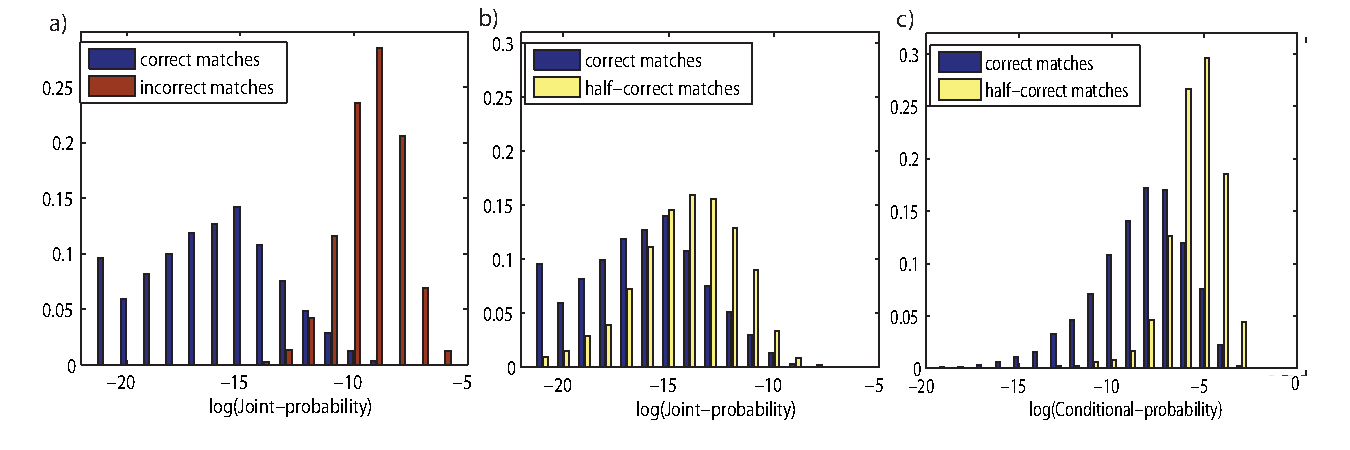
\includegraphics[height=40mm, width=120mm]{figures/MixGF_separation_true_false_matches.eps}
		\caption{Separating true matches from false matches:
		Mixture spectra were simulated by a linear combination of two single-peptide spectra. For each mixture spectrum we extracted the correct match as well the top-scoring incorrect and half-correct matches returned by MixDB.  Correct matches are cases where both peptides in a Peptide-Peptide Spectrum Match (PPSM) are correct; incorrect matches are cases where both peptides are incorrect and half-correct matches are cases where one peptide is correct and one peptide is incorrect. The distribution of Joint-probability and Conditional-probability for correct matches (blue bars) incorrect matches (red bars) and half-correct matches (yellow bars) are shown.  As shown in a), the distributions of Joint-probability are well-separated between correct and incorrect matches. However, there is considerable overlap between the Joint-probability distribution of correct matches and half-correct matches (see b).  On the other hand, Conditional-probability is a better feature for separating correct matches from half-correct matches as shown in c).}
\label{separate}
\end{figure}

\subsection*{Approximating joint by product of conditional probability}
Although Joint and Conditional-probability are good features that separate correct matches from incorrect matches and half-correct matches, the calculation of Joint-probability involve computing a three-dimensional dynamic programming table, which is computationally expensive (it takes minutes to compute the Joint-probability for each spectrum).  Moreover, this approach cannot easily scale to mixture spectra from more than two peptides as the computational cost grows exponentially with the number of peptides.  Thus rather than computing the Joint-probability exactly, we seek to approximate it by a product of Single-peptide probability and Conditional-probability, both of which can be computed efficiently.  Using our simulated mixture spectra dataset, we compare the Joint-probability and its approximation.  As shown in Figure~\ref{approximate}, for most cases the Joint-probability is approximated quite accurately as most data points clustered tightly along the main diagonal line.  For correct matches, the approximation sometimes underestimates the Joint-probability.  This can be attributed to the fact that in the approximation we did not explicitly consider all the dependencies between the two peptides.  However, the range of probabilities where this underestimation occurs is well below the range where incorrect matches tends to occur.  Therefore for the purpose of separating correct matches from incorrect matches, using the approximation is nearly equivalent to computing the exact Joint-probability. As shown in Figure \ref{approximate}b, correct matches and incorrect matches remain very well-separated whether using the Product or Joint-probability.

\begin{figure}
	\centering
	 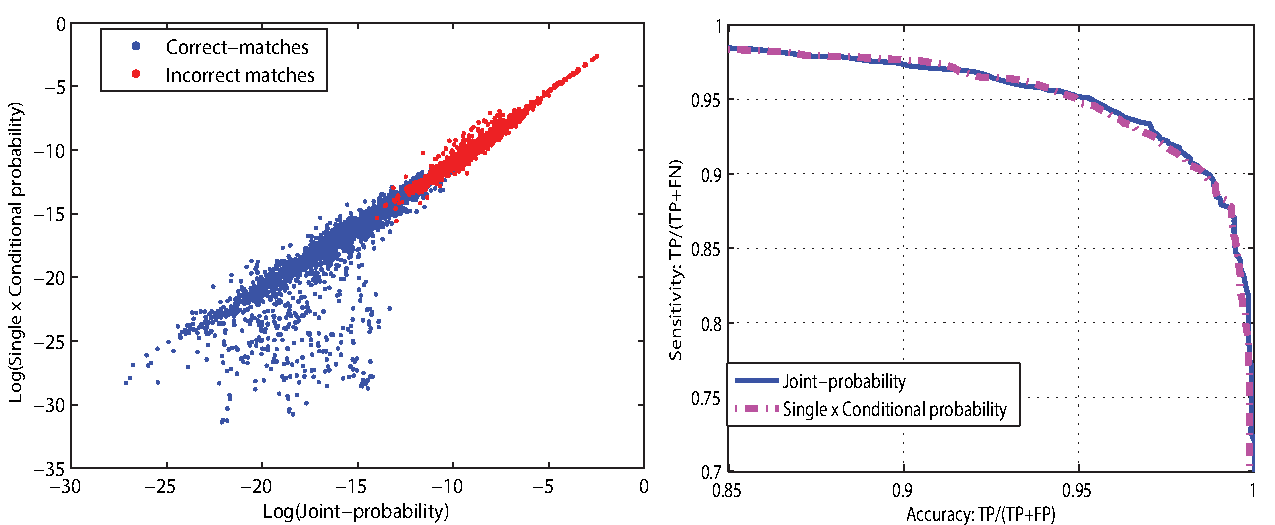
\includegraphics[height=50mm, width=120mm]{figures/MixGF_approx_joint_by_product_distrib_plus_ROC.eps}
		\caption{Approximation of Joint-probability:
	It is computationally expensive to compute the exact Joint-probability for a mixture spectrum because it scales exponentially with the number of peptides considered. We thus evaluate approximating Joint-probability by the product of Single-peptide and Conditional probability, both of which can be computed in linear time. As shown in a): for most cases we are able to accurately approximate the Joint-probability (most data points cluster tightly around the main diagonal).  For correct-matches, there are some cases falling below the main diagonal. This shows that the approximation sometimes underestimates the true Joint-probability for correct matches.  However, for the practical purpose of distinguishing correct-matches and incorrect-matches, the two distributions remain very well separated using either the exact Joint-probability or its approximation as shown in the ROC curve on the right.}
\label{approximate}
\end{figure}

\subsection*{MixGF increase the sensitivity of identification of mixture spectra}
%To compare MixGF with existing methods in identifying mixture spectra, we compare MixGF with the SVM-scores used by MixDB at separating true and false matches in the simulated mixture spectra dataset.  As shown in Figure~\ref{improve}, MixGF is able to identify 20-30\% more mixture spectra at various different FDR level.

%\begin{figure}
%	\centering
%	 \includegraphics[height=50mm, width=100mm]{figures/MixGF_vs_MixDB_ROC.eps}
%		\caption{MixGF improve sensitivity of identifying mixture spectra
%		In a set of simulated mixture spectra, we compare the performance of identifying mixture spectra using MixDB and MixGF. As shown in figure, MixGF
%improve the sensitivity of identifying mixture spectra by 20-30\% accross a range of different false discovery rate (FDR) threshold.
%}
%\label{improve_mixture}
%\end{figure}

To benchmark MixGF's ability to identify mixture spectra, we tested it on a Yeast dataset~\cite{li2009} that represents a typical proteomics experiment and has been shown in previous studies to contain many mixture spectra~\cite{wang2010msplit}.  We compared the performance of MixGF with two current state-of-the-art database search methods for identification of mixture spectra: MixDB and ProbIDtree. As shown in Table~\ref{tab:compare}, MixGF is able to outperform MixDB and ProbIDtree by identifying 26-76\% and 110-162\%
%30\% and 90\% 
more mixture spectra at the same FDR, respectively.  We also compared different variants of MixGF in which a different probability function was used at stage one to separate correct matches from incorrect matches.  They are all followed by using Conditional-proability at the second stage to separate correct matches from half-correct matches.  Note that the performance when using the Joint-probability and its approximation ( Product-probability) is very similar, further indicating that our approximation of the joint proability is sufficiently accurate as a score for FDR-controlled identifications.  One exception to that is at 1\% FDR, using Joint-probability at the first stage identifies more mixture spectra than Product-probability. We note that this might be due to an artifact of using TDA to estimate FDR since at 1\% FDR, there can be only a very small number (i.e. 5-13 spectra) of decoy mixture spectra allowed to pass the FDR threshold.  Thus a small random fluctuation in the number of decoy spectra passing the FDR threshold results in a relative large change in FDR estimation.  As we allow for slightly higher FDR (such that small fluctuations in the numbers of decoy spectra passing the FDR threshold no longer significantly influence the FDR estimation) we see that using Joint-probability and Product-probability results in very similar performance.
\vspace{-3mm}
\begin{table}
	\begin{center}
	  \begin{tabular}{p{5cm}|p{1.2cm}p{1.2cm}p{1.2cm}p{1.2cm}p{1.2cm}} % centered columns (4 columns)
			\hline
              & \multicolumn{5}{c}{False discovery rate (FDR)} \\
			 % & Single-peptide & Mixture & Total & Single-peptide & Mixture & Total\\
			      & 1\%  & 2\% & 3\% & 4\% & 5\%  \\
  			\hline
  			\noalign{\smallskip}
  			ProbIDtree & 504  & 773  & 923 & 1029  & 1272 \\
  			MixDB      & 748 & 1214 & 1620 & 1905 & 2124  \\
  			MixGF (Joint-probability) & 1320 & 1580 & 1972 & 2268 & 2676 \\
  			MixGF (Product-probability) & 1011 & 1646 & 2038 & 2356 & 2688 \\
			  MixGF (Single-peptide probability) & 1310 & 1664 & 2091 & 2452 & 2760\\
			 \hline
		\end{tabular}
  \end{center}
		%*SpectraST results after adjusting F-score threhold to bring SpectraST precision to 97\% \\as estimated for the other methods.\\
	\caption{Numbers of mixture spectra identified in the Yeast dataset by ProbIDtree, MixDB and MixGF are shown.  The different variants of MixGF differ by the probability (indicated in parenthesis) that is used in the first stage to separate correct matches from incorrect matches.  It is always followed by using Conditional-probability in the second stage to separate correct matches from half-correct matches.}
	\label{tab:compare}
\end{table}
\vspace{-5mm}

It is perhaps somewhat surprising that using Single-probability has comparable performance to using Joint-probability.  For mixture spectra, we expect Joint-probability to perform better at separating \emph{correct matches} from \emph{incorrect matches} by explicitly considering two peptides. Intuitively we expect that Single-peptide probabilities for correct peptide matches to mixture spectra to be higher (i.e. worse) than those for correct matches to single-peptide spectra.  This is because the presence of a second peptide in mixture spectra which will allow more peptides to match to the spectrum with high score. However for false matches the single-peptide probability distribution remains roughly the same for both single-peptide and mixture spectra because they are random matches in either case.  Therefore the distribution of Single-peptide probabilities between correct and incorrect matches should be less well-separated for mixture spectra than for single-peptide spectra.  Further analysis shows that this can be explained by the fact that in the Yeast dataset, most mixture spectra have the second peptide at relatively low abundance (we estimated that on average, the low-abundance peptides are at $1/3$ of the intensity of the high-abundance peptides~\cite{wang2010msplit}).  When the second peptide in the mixture is at relatively low abundance, the mixture spectrum tends to be more similar to a single-peptide spectrum and thus the ability to separate \emph{correct} from \emph{incorrect matches} using either Joint or Single-peptide probability is similar in these cases.  To show this we generated a series of simulated mixture spectra where the first peptide is mixed with a second peptide at 100\%, 50\%, 30\% of the first peptide's total intensity and then computed the Single-peptide probability, Joint-probability and Product-probability for the correct matches as well as the top-scoring incorrect matches. The performance of each probability function in separating correct from incorrect matches is shown in Table~\ref{tab:mixgf_stage1}.  As expected when the second peptide is at relatively low abudance (i.e. 30\%), the performance of Single-peptide and Joint-probability is similar. However as we increase the relative abundance of the second peptide, Joint-probability performs considerably better at separating correct matches from incorrect matches.  Thus we expect that as mixture spectra with more peptides become more common in proteomic experiments, Joint-probability and its approximation will substantially improve our ability to identify mixture spectra.
%We noted that this characteristic may be associate with the particular dataset that is being used here. The Yeast dataset maybe of limited complexity in the sense there are may not be many co-eluting peptides.  In cases where more complex sample mixture are being analyzed or in data-independent-acquisition strategy where multiple precursors are selected for co-fragmentation, we expected the joint-probability and its approximation will increase the sensitivity of identifying mixture spectra.
\vspace{-2mm}
\begin{table}
	  \centering
		\begin{tabular}{p{3cm}|p{3cm} p{1.5cm} p{1.5cm} p{1.5cm}} % centered columns (4 columns)
			\hline
        Mixture Coefficient & Probability  & \multicolumn{3}{l}{False discovery rate (FDR)} \\
			          &               & 1\%  & 2\% & 5\% \\%& 10\%  \\
  			\hline \noalign{\smallskip}
  			$\alpha=1.0$ & Single-probability  & 71.9 & 74.7 & 81.8 \\%& 86.8 \\
  			             & Joint-probability   & 93.4 & 94.7 & 96.6 \\%& 97.6 \\
  			             & Product-probability & 93.6 & 94.0 & 96.7 \\%& 98.1 \\
  		  \hline \noalign{\smallskip}
  			$\alpha=0.5$ & Single-probability  & 85.7 & 87.5 & 92.0 \\%& 93.9 \\
  			             & Joint-probability   & 93.5 & 94.3 & 96.0 \\%& 98.1 \\
  			             & Product-probability & 92.6 & 94.1 & 96.1 \\%& 97.9 \\
  			\hline \noalign{\smallskip}
  			$\alpha=0.3$ & Single-probability  & 89.4 & 90.8 & 92.8 \\%& 93.8 \\
  			             & Joint-probability   & 90.2 & 91.8 & 93.8 \\%& 95.3 \\
  			             & Product-probability & 90.4 & 91.7 & 93.8 \\%& 95.6 \\
  			\hline
		\end{tabular}
		\caption{Sensitivity of accepting correct mixture spectrum matches at stage one of MixGF with different probabilities.
		A set of simulated mixture spectra were constructed with mixture coefficient $\alpha=1.0, 0.5, 0.3$ respectively.
		Single-probability, joint-probability and product-probability were computed for the correct matches as well as the top-scoring
		incorrect matches returned by MixDB. Then each probability was used to separate correct from incorrect
		matches.  The sensitivity of accepting correct matches at different FDR levels is shown.}
	%The numbers of single-peptide as well as mixture spectra and total numbers of unique peptides identified are compared.
	\label{tab:mixgf_stage1}
\end{table}
\vspace{-2mm}
\section*{Discussion}
As is clear from the trends in mass spectrometry instrumentation (e.g SWATH, QExactive, IMS, MS$^{E}$\cite{masselon2003itp,venable2004aaq,plumb2006uplc,chakraborty2007uim,panchaud2009precursor,michalski2011mass,2012targeted}) \emph{mixture} MS/MS spectra from more than one peptide are rapidly becoming very common since these technologies allow for the reproducible and sensitive analysis of increasingly complex biological samples.  These methods have the potential to provide a more complete and quantitative view of the proteome. However this will also require the development of computational tools that can accurately identify multiple peptides in each MS/MS spectrum.  Two fundamental questions need to be addressed in order to deliver accurate identification tools: 1) to separate correct multiple-peptide-spectrum matches (mPSMs) from false positive matches and 2) to estimate the false discovery rate in a set of mPSMs.  Here we address the first question by computing the statistical significance of mPSMs. Given an MS/MS spectrum, database search tools can always return a top-scoring peptide or peptides matched to the query spectrum. By random chance it is always possible for some false peptide matches to obtain a high score.  This is especially true for mixture spectra because of the exponential explosion in the size of the search space.  Thus it is crucial to be able to accurately compute the random chance that an mPSM with a particular score T can occur.  Here we showed that for the two-peptide case, it is possible to compute such probabilities rigorously using a generating function approach and show that Joint and Conditional-probabilities are very good features that can separate correct from false positive matches.  In addition we further show that the computationally expensive Joint-probability can be approximated accurately using a product of Single and Conditional-probabilities, each of which can be computed in linear time.  In order to estimate the false discovery rate (FDR) for mixture spectra, we extend the traditional target-decoy approach (TDA).  We note that it is essential to perform the database search using a concatenated target-decoy sequence database as this allows one to model and estimate the occurrence of half-correct matches where one peptide in the PPSM is correct and the other peptide is incorrect.  This is important because these constitute a much larger fraction of false positive matches in mixture spectra than cases where both peptides are incorrect and as we show here these cases are more difficult to separate from correct matches.  Finally even though our focus was on mixture spectra from two peptides, this assumption is not required in our approach and thus MixGF should be readily extensible to cases with more than two peptides.  Focusing on a relative simple case allowed us to comprehensively assess various performance and computational efficiency aspects of our approach.  Benchmarking on simulated as well as real dataset shows that our new approach is able to identify 26\%-162\% more mixture spectra than current state-of-the-art database search tools for identification of mixture spectra.

\section*{Acknowledgments.} The authors would like to thank NIST, ProteomeCommons and Vanderbilt University for the public availability of the mass spectrometry data used in this research.  This work was partly supported by the National Institutes of Health grant GM078596 (JW and PEB) and 1-P41-RR024851 (NB) from the National Center for Research Resources.

\clearpage
\bibliographystyle{unsrt}
\bibliography{./msms}
\end{document}
